% !TeX root = ../main.tex

\section{Intro}
\subsection{Numerical Analysis and Errors}
M = Math\\
CS = Computer Science\\
E = Engineering

Numerical Analysis = M$\cap$CS\\
Basic methods to approach math problems

Scientific Computing = M$\cap$CS$\cap$E
Take a problem and replicate it on a digital device to understand better the situation

\begin{figure}[!ht]
    \begin{minipage}{\linewidth}
        \centering
        \makebox[\textwidth][c]{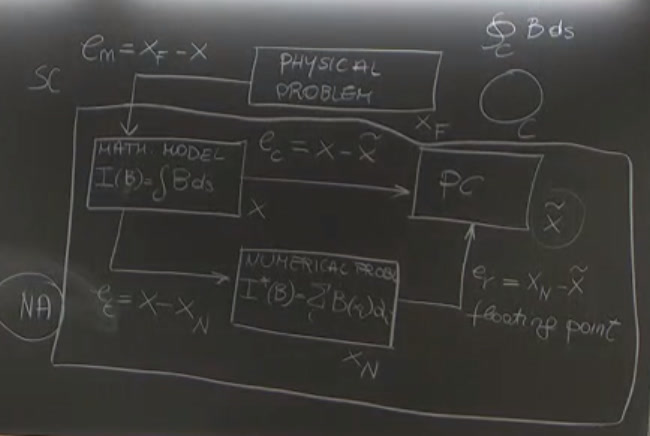
\includegraphics[width=1\textwidth]{images/Screenshot from 2022-09-21 15-28-17.png}}%
    \end{minipage}
\end{figure}
Where:
$$
\begin{cases}
    x_F\text{ solution of physical model}\\
    x\text{ solution of mathematical model}\\
    \tilde{x}\text{ does not substitute reality simulation}\\
\end{cases}
$$
We replaced the integral with a summation, ia PC there is no concept of infinity.\\
What to do after we observe what's going on? Use a better model or a better $x\leftrightarrow\tilde{x}$ mapping.

Errors:
$$
\begin{cases}
    e_m=x_F-x\text{ modelling error between physical problem and mathematical model}\\
    e_c=x-\tilde{x}\text{ computational error}=e_t+e_r
    \begin{cases}    
        e_t=x-x_N\text{ truncation error}\\
        e_r=x_N-\tilde{x}\text{ rounding error, floating point approximation}
    \end{cases}
\end{cases}
$$

Kinds of errors:
\begin{itemize}
    \item $|x-\tilde{x}|$\\
    \textbf{Absolute error}, $|e_c|$. Consider absolute error based on model
    \item $\frac{|x-\tilde{x}|}{|x|}$\\
    \textbf{Relative error}, more meaningful, like percentage
\end{itemize}

\subsection{Floating point representation}